\documentclass[10pt]{article}
\usepackage{float}
\usepackage{listings}
\usepackage[french]{babel}
\usepackage[utf8x]{inputenc}
\usepackage{subcaption}
\usepackage{listings}
\usepackage{wrapfig}
\usepackage{color}
\usepackage{amsmath}
\usepackage{amsfonts}
\usepackage{mathtools}
\usepackage{graphicx}
\usepackage{caption}
\definecolor{dkgreen}{rgb}{0,0.6,0}
\definecolor{gray}{rgb}{0.5,0.5,0.5}
\definecolor{mauve}{rgb}{0.58,0,0.82}
%opening

\lstset
{frame=tb,
	language=R,
	aboveskip=3mm,
	belowskip=3mm,
	showstringspaces=false,
	framexleftmargin=5mm,
	columns= fixed,
	numbers = left,
	basicstyle={\small\ttfamily},	
	numberstyle=\tiny\color{gray},
	keywordstyle=\color{blue},
	commentstyle=\color{dkgreen},
	stringstyle=\color{mauve},
	breaklines=true,
	breakatwhitespace=true,
	tabsize=3
}


\title{
	\normalfont \normalsize 
	\textsc{Université de Technologie de Compiègne\\ 
		SY09:Analyse des données et Data-Mining , P17} \\
	[10pt] 
	\rule{\linewidth}{0.5pt} \\[6pt] 
	\huge Premier Rendu \\
	\rule{\linewidth}{2pt}  \\[10pt]
}
\author{Oumaima Talouka, Zineb Slam}
\date{\normalsize \today}

\begin{document}
	
	{\let\newpage\relax\maketitle}
	
	Dans ce rapport du TP1 de l'UV SY09 nous allons expliquer notre démarche dans l'analyse des données en expliquant les résultats obtenus. Ce TP est composé de 2 parties. La première partie a pour objectif de se familiariser avec les méthodes de traitement et de visualisation de données sur R. La deuxième partie traite de l'Analyse en composantes principales (ACP). Nous allons travailler avec 3 datasets: notes de SY02, Crabs et Pima qu'on va d'abord analyser et décrire avant d'y réaliser l'ACP en seconde partie. Pour les graphes obtenus nous avons utilisés la librairie ggplot2 qui offre un grand nombre de fonctionnalités. Le code R sera fourni en annexe.
	
	
	
	
	\section{ Statistique descriptive}
	
	\subsection{Notes SY02}
	Le dataset \textit{"sy02-p2016"} représente les notes des étudiants de l'UTC en méthodes statistiques durant le printemps 2016. Nos données comptent \textit{N= 296} individus (étudiants) er \textit{p= 11} variables. Nous avons omis  les étudiants qui n'avaient pas de résultats (\textit{NA}) ou qui ont '\textit{ABS}' en résultat de l'UV parce que ce qu'on a pensé que ce sont des étudiants qui s'étaient désinscris ou n'ont pas suivi l'UV et donc ne constituent pas d'information pour notre dataset. Nous gardons néanmoins les étudiants qui ont NA en médian ou en final mais qui ont obtenu un résultat final. 
	
	\begin{lstlisting}
	dataset = dataset[!is.na(dataset$resultat), ]
	dataset = dataset[dataset$resultat!='ABS', ]
	\end{lstlisting}
	
	Nous gardons donc \textit{N = 284} individus pour notre étude.
	
	\subsubsection{Description des variables}
	
	
	\begin{itemize}
		\item \textbf{Variables Quantitatives}: note.median, note.final et  note.totale.
		\item  \textbf{Variables Qualitatives Nominales}: nom, specialite, status, dernier.diplome.obtenu et correcteur.median, correcteur.final
		\item  \textbf{Variables Qualitatives Ordinales}: niveau et resultat  \\
	\end{itemize}
	Nous allons a présent définir  chaque variable en précisant son intervalle ou les valeurs qu'elle peut prendre.
	
	\begin{itemize}
		\item \textbf{Nom:} chaine de caractère identifiant chaque étudiant.
		\item \textbf{Spécialité:} la branche de l'étudiant: \textit{GB}, \textit{GM}, \textit{GSM}, \textit{GP} et \textit{GI}.
		\item \textbf{Niveau}: Semestre d'étude de chaque étudiant de 1 a 6.
		\item \textbf{Statut}: Soit l'étudiant est de l'\textit{UTC} ou en \textit{semestre d'échange}
		\item \textbf{dernier.diplome.obtenu:}
		\textit{BAC, DUT, CPGE, ETRANGER SUPERIEUR, LICENCE, OTHER, NA}
		\item \textbf{Note Médian:} note de l'examen Médian, ensemble de réel de 0 a 20.
		\item \textbf{Correcteur Médian:} ID du correcteur du médian \{Corr1, Corr2, Corr4., Corr5,..,Corr8\}
		\item \textbf{Note.final:} Note de l'examen final, ensemble de réel de 0 a 20.
		\item \textbf{Note.totale:} Note totale obtenue a partir de la note du médian et la note du final
		\item \textbf{Correcteur.final}: identifiant  du correcteur du final. \{Corr1..Corr3, Corr4., Corr5,..,Corr8\}
		\item \textbf{Résultat}: Résultat obtenu en SY02 : \textit{A, B, C, D, E et FX et FX. ABS}. ABS est pour indiquer que l'étudiant était absent pour l'examen en question.
	\end{itemize}
	
	Pour les notes de médian et de final, il y a des notes non mentionnées (NA), par contre tous les étudiants ont un résultat final c'est pour cela que nous n'avons pas enlevé les étudiants avec NA en médian ou/et en final.\\
	Les variables importantes dans ce dataset sont les résultats des étudiants et comment ceux-ci sont influencés par d'autres variables, par exemple le niveau et la spécialité\\
	Il est évident qu'il existe une relation linéaire entre ces 3 variables: note.median, note.final et note.totale vu que la note totale est exprimée par une relation linéaire entre la note.median et la note.final (par exemple $note.totale = 40\% * note.median + 40\% * note.final + cste$). La variable note.totale et la variable résultat sont des variables fortement corrélées. En effet, le résultat est une "traduction" de la note totale. On pourrait éventuellement se demander sur la relation entre les notes et le niveau, la spécialité, le diplôme ainsi que le correcteur. C'est ce que nous allons essayer d'analyser dans ce qui suit. 
	
	\subsubsection{Liens entre les variables}
	Après avoir représenté la matrice de graphes pour chaque variable nous avons pu observé que les variables : note.median, note.final, et note.totale sont linéaires, ce qui confirme notre hypothèse précédente. Le graphe matriciel ci-dessous présente aussi les coefficients de corrélation entre chacune de ces variables.
	
	\begin{center}
		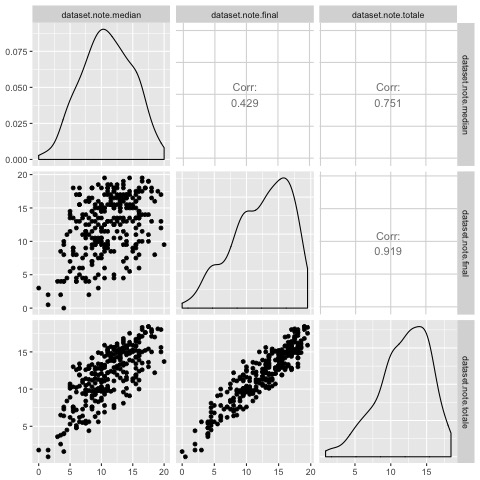
\includegraphics[width=50mm]{Figures/Notes/corr_notes.jpg}
		\captionof{figure}{Plot général}
		\label{fig:multiplot_notes}
	\end{center}
	
	
	\subsubsection{Homogénéité et Distribution des notes}
	La figure ci-dessous représente trois diagrammes en boîtes des notes de médian, final et le résultat de l'UV SY02. 
	
	\begin{minipage}{.4\textwidth}	
		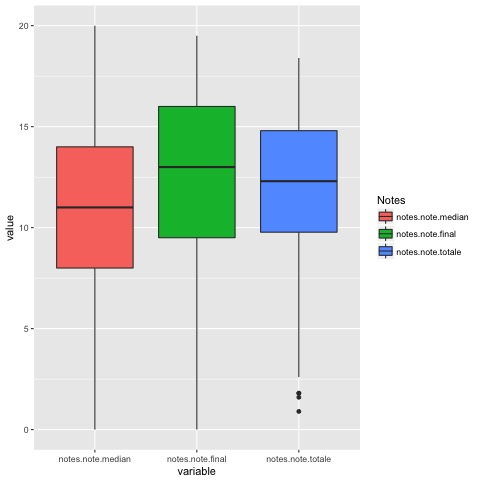
\includegraphics[width=55mm]{Figures/Notes/boxplot_exam.jpg}
		\captionof{figure}{Boxplot des Notes }
		\label{fig:Boxplot_notes}
	\end{minipage}%
	\hspace{0.03\linewidth}
	\begin{minipage}{.6\textwidth}
		\begin{tabular}{ c c c c }
			\textbf{}       & \textbf{Médian} & \textbf{Final}   & \textbf{Total} \\
			\textbf{1er Quartl}    & 8.0 			       & 9.50		      & 9.77    \\
			\textbf{Médiane  }   &11.0		             & 13.0	            & 12.3    \\
			\textbf{Moyenne}     & 10.92                &  12.38          & 11.84\\
			\textbf{3em Quartl}  & 14.0  				& 16.0 		       & 14.8\\
		\end{tabular}
	\end{minipage}
	
	
	On remarque que les boîtes sont petites, ce qui laisse penser que la variance des résultats est relativement petite et donc aussi que le niveau des étudiants en statistiques l'est aussi.  En comparant les diagrammes du final et du médian on remarque que les notes ont augmenté.  Enfin si on analyse le dernier diagramme, on voit que les deux boîtes de part et d'autre de la médiane ont la même taille. Nous pouvons donc émettre l'hypothèse que les résultats sont normalement distribués. 
	
	Il est tout a fait logique que le diagramme en boîtes des notes finales se situe entre les 2 puisque la note finale est une moyenne des deux notes du médian et du final.
	
	
	\subsubsection{Lien entre la réussite, la formation, la branche et le niveau}
	Comme les étudiants de chaque branche n'ont pas les \textit{même effectifs}, nous avons choisi de représenter les données sous forme de diagrammes à moustaches pour mieux pouvoir les comparer.\\
	
	
	\begin{minipage}{.5\textwidth}
		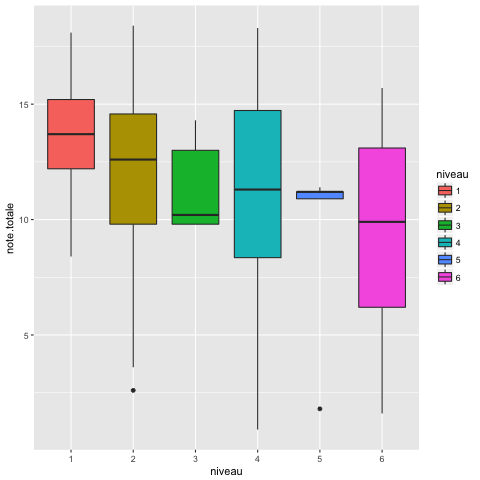
\includegraphics[width=50mm]{Figures/Notes/niveau_resultat.png}
		\captionof{figure}{Diagramme en boîtes de lien entre le niveau et le résultat}
		\label{fig:niveau_resultat}
	\end{minipage}%
	\hspace{0.08\linewidth}
	\begin{minipage}{.5\textwidth}
		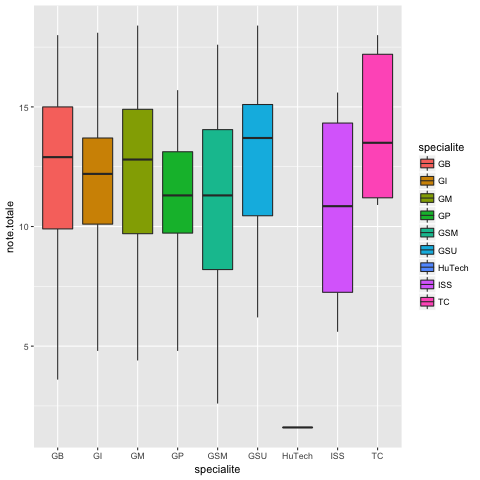
\includegraphics[width=50mm]{Figures/Notes/specialite_resultat.png}
		\captionof{figure}{Diagramme en boîtes de entre la branche et le résultat}
		\label{fig:specialite_resultat}
	\end{minipage}
	D'après la figure \ref{fig:niveau_resultat} on remarque que les étudiants venant durant les premiers semestres sont ceux qui réussissent le mieux leur examens de SY02 , suivi par ceux en GX02. On remarque que les notes des étudiants en GX04 et GX05 ont une grande variance. Les étudiants en GX04 et en GX05 ont . Il faut aussi remarquer que les étudiants en 4eme et 5eme sont peu comme ce sont des semestres de départ en stage. \\
	En ce qui concerne l'influence de la spécialité sur les notes on remarque qu'il y'a une grande variance dans les notes chez les étudiants en TC, ISS et GSM, contrairement au GI et GP qui ont plutôt un niveau homogène et qui semblent bien réussir l'UV. De plus les TC sont aussi ceux qui réussissent le mieux l'UV.
	\begin{center}
		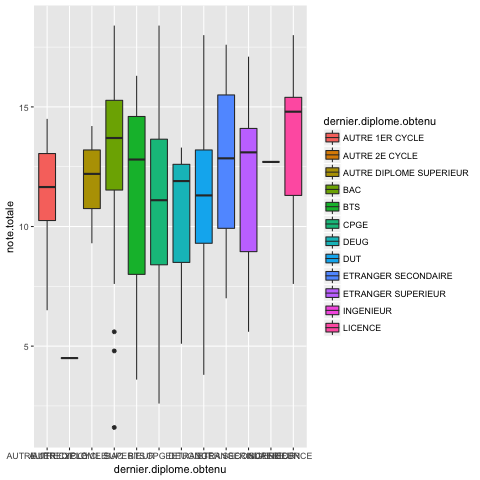
\includegraphics[width=50mm]{Figures/Notes/diplome_resultat.png}
		\captionof{figure}{Diagramme à moustaches du lien entre la formation et le résultat}
		\label{fig:formation_resultat}	
	\end{center}
	
	On remarque qu'il y a une grande variance chez presque tous les diplômes obtenus. Les élèves qui réussissent le mieux et le plus sont ceux provenant de la Licence.  Plus de 75\%  (\textbf{Check}) des etudiants de autre premier  cycle et autres diplômes et du BAC réussissent l'UV SY02. En ce qui concerne les résultats des étudiants pour le reste des diplômes, ils ont une grande variance et ne sont pas normalement distribués. En particulier les étudiants du BTS, CPGE et du DEUG sont ceux qui ont la plus grande variance et le plus grand échec.
	
	
	\subsubsection{Influence du correcteur sur la note}
	
	\begin{minipage}{\linewidth}
		Les deux diagrammes ci-dessous montrent la dispersion des notes de final et de médian pour chaque correcteur.\\
		\begin{minipage}{0.50\linewidth}
			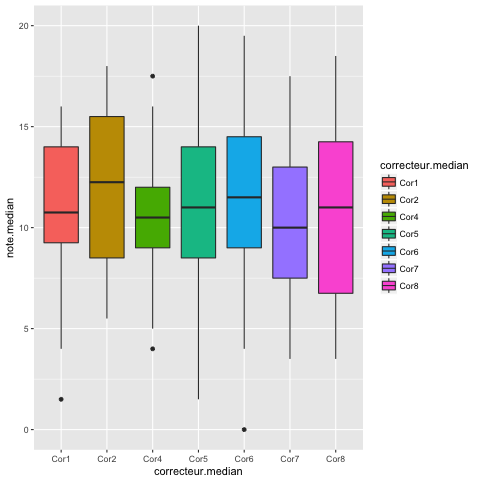
\includegraphics[width=50mm]{Figures/Notes/correcteur_median.png}
			\captionof{figure}{Diagramme à moustaches des notes de médian en fonction des correcteurs}
			\label{fig:scatter_correcteur_median}
		\end{minipage}
		\hspace{0.01\linewidth}
		\begin{minipage}{0.50\linewidth}	
			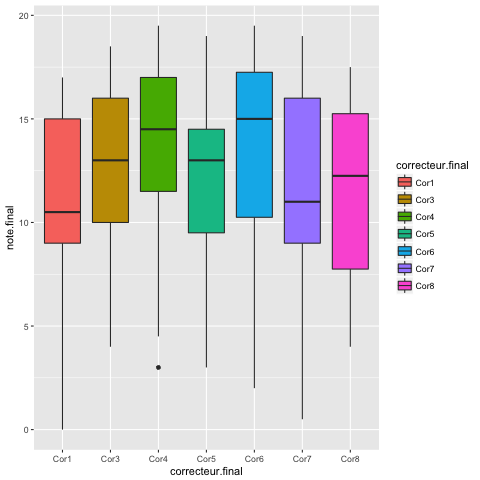
\includegraphics[width=50mm]{Figures/Notes/correcteur_final.png}
			\captionof{figure}{Diagramme à moustaches des notes du final en fonction des correcteurs}
			\label{fig:scatter_correcteur_median}
		\end{minipage}
	\end{minipage}
	on considère que les copies sont aléatoirement distribuées pour chaque correcteur et donc il n'y a pas de correcteur qui a que les 'bons' ou les 'mauvais' étudiants. A première vue on remarque qu'en général les notes sont dispersées pour chaque correcteur et donc il n'y a pas vraiment de correcteur en particulier qui semble être plus 'sévère' que les autres. On peut émettre l'hypothèse que le \textit{Corr4} a été plus stricte dans ses corrections de médians, néanmoins son diagramme de notes de final prouve le contraire. Il se peut donc que le correcteur ait eu les copies des 'mauvais' étudiants par fruit de hasard. Finalement, comme il a été cité précédemment les notes ont augmenté au final par rapport au médian, on observe donc bien que ceci est le cas pour tous les correcteurs.
	
	\subsubsection{Conclusion}
	Cette première analyse data nous a permis d'étudier quels sont les facteurs qui influent sur la réussite d'un étudiant dans l'UV SY02 comme le dernier diplôme obtenu ou le niveau et ceux qui n'influencent pas comme le correcteur. Néanmoins ces conclusions sont \underline{propre à la population du P16} et donc  \underline{biaisées}; pour pouvoir généraliser il faut analyser les notes de SY02 sur plusieurs semestres avec des populations différentes.
	
	\subsection{Crabs}
	Le dataset \textit{"Crabs"} représente un jeu de données de 200 crabes décrits par huit variables, trois sont qualitatives et cinq sont quantitatives.
	
	\subsection{Description des variables}
	
	
	\begin{itemize}
		\item \textbf{Variables Qualitatives Nominales :}  crabs.sp, crabs. sex, crabs.inde
		\item \textbf{Variables Quantitatives : } crabs.FL, crabs.RW, crabs.CL, crabs.CW, crabs.BD
	\end{itemize}
	
	Nous pouvons représenter les données des variables quantitatives a l'aide un boxplot.
	\begin{center}
		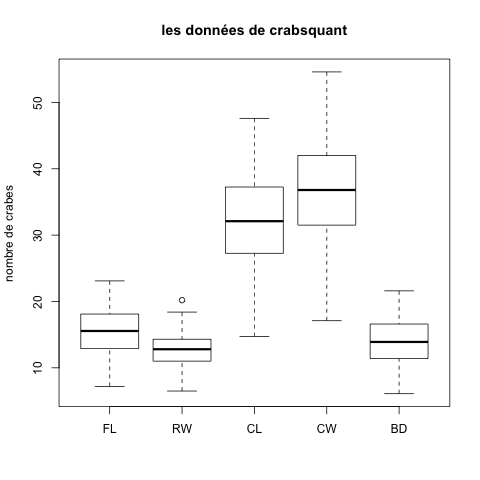
\includegraphics[width=50mm]{Figures/Crabs/bxp_crabsquant.png}
		\captionof{figure}{Boxplot des données quantitaves}
		\label{fig:boxplot_crabs_quantitatives}
	\end{center}
	
	Nous remarquons d'ores et déjà que deux catégories de variables se distinguent, d'un cote FL, RW et BD et d'un autre, CL et CW.
	
	Avant de continuer l'analyse de ces données, nous pouvons préciser la signification de chacune de ces variables comme suit:
	\begin{itemize}
		\item \textbf{sp:} \textit{(species)}, espèce, "B" pour Bleu et "O" pour Orange
		\item \textbf{sex:} sexe, "F" pour Femelle et "M" pour Mâle
		\item \textbf{index:} index de 1 a 50 pour chacune des 4 catégories suivantes : \{"B,M","O,M","B,F","O,F"\}
		\item \textbf{FL:} Frontal Lobe size en mm
		\item \textbf{RW:} Rear Width en mm
		\item \textbf{CL:} Carapace Length en mm
		\item \textbf{CW:} Carapace Width en mm 
		\item \textbf{BD:} Body Depth en mm
	\end{itemize}
	
	\subsection{Analyse descriptive des données}
	
	\subsubsection{Représentation de chaque caractéristique en fonction de l'espèce}
	
	Afin de voir s'il y a une différence de caractéristiques morphologiques en fonction de l'espèce d'abord, nous représentons les boîtes à moustaches de chaque variable morphologique en fonction de la variable \text{sp} comme suit:
	
	\begin{center}
		\begin{minipage}[t]{0.3\textwidth}
			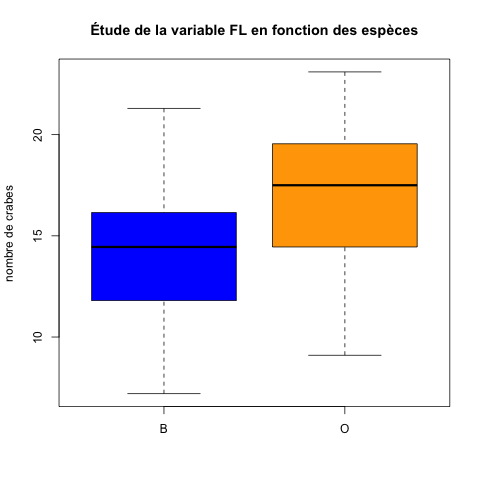
\includegraphics[width=35mm]{Figures/Crabs/bxp_sp_fl.png}
		\end{minipage}
		\begin{minipage}[t]{0.3\textwidth}
			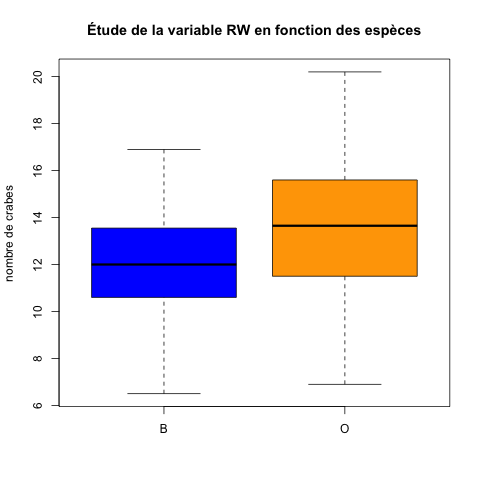
\includegraphics[width=35mm]{Figures/Crabs/bxp_sp_rw.png}	
		\end{minipage}
		\begin{minipage}[t]{0.3\textwidth}
			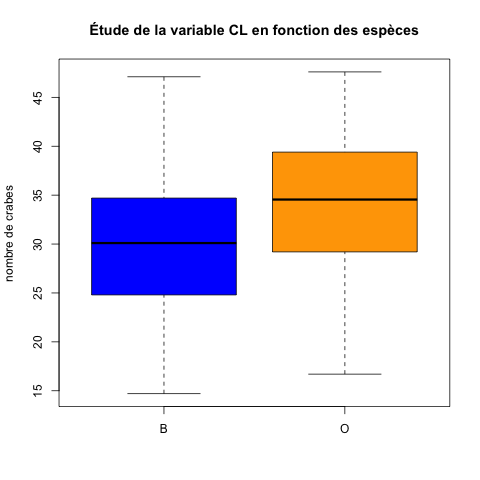
\includegraphics[width=35mm]{Figures/Crabs/bxp_sp_cl.png}
		\end{minipage}
		\newline
		\begin{minipage}[t]{0.3\textwidth}
			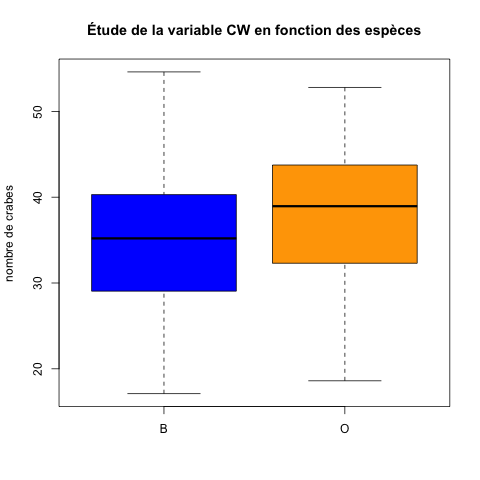
\includegraphics[width=35mm]{Figures/Crabs/bxp_sp_cw.png}	
		\end{minipage}
		\begin{minipage}[t]{0.3\textwidth}
			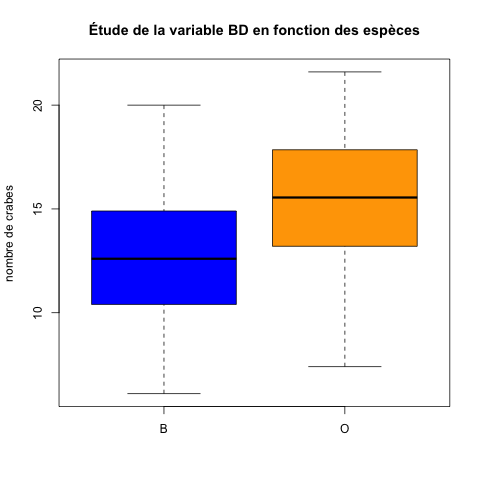
\includegraphics[width=35mm]{Figures/Crabs/bxp_sp_bd.png}
		\end{minipage}
	\end{center}
	
	Il y a des distributions assez différentes en fonction de l'espèce. Les intervalles de confiances ne se chevauchent pas. Cependant, la dispersion des données reste assez homogène au vue des boxplots.
	\subsubsection{Représentation de chaque caractéristique en fonction du sexe}
	
	Afin de voir s'il y a une différence de caractéristiques morphologiques en fonction du sexe, nous représentons les boîtes à moustache de chaque variable morphologique en fonction de la variable \textit{sex} comme suit:
	
	\begin{center}
		\begin{minipage}[t]{0.3\textwidth}
			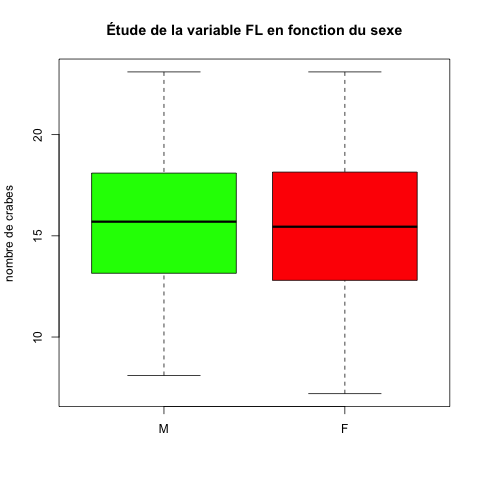
\includegraphics[width=35mm]{Figures/Crabs/bxp_sex_fl.png}
		\end{minipage}
		\begin{minipage}[t]{0.3\textwidth}
			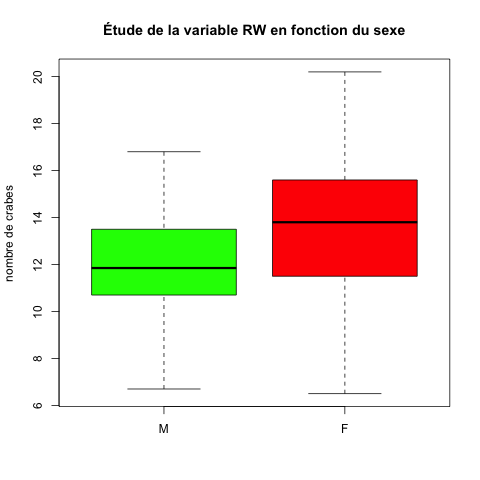
\includegraphics[width=35mm]{Figures/Crabs/bxp_sex_rw.png}	
		\end{minipage}
		\begin{minipage}[t]{0.3\textwidth}
			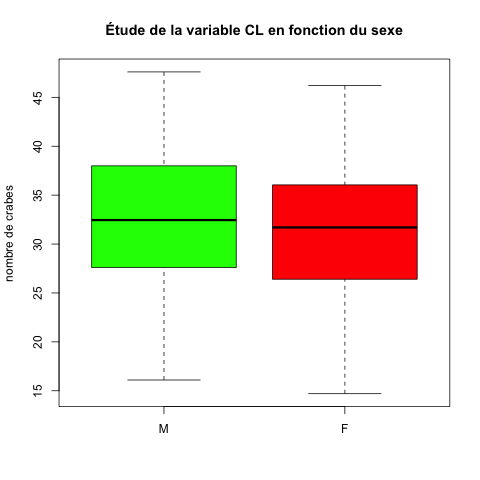
\includegraphics[width=35mm]{Figures/Crabs/bxp_sex_cl.png}
		\end{minipage}
		\newline
		\begin{minipage}[t]{0.4\textwidth}
			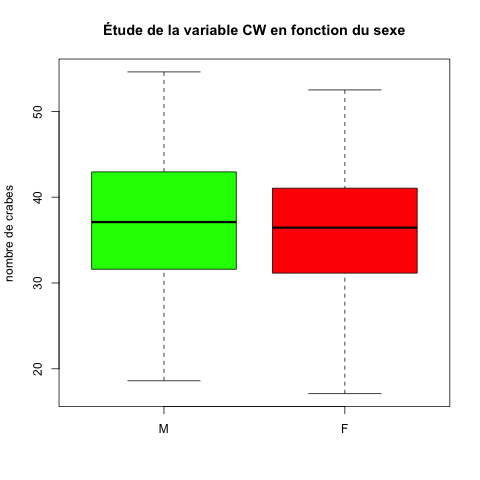
\includegraphics[width=35mm]{Figures/Crabs/bxp_sex_cw.png}	
		\end{minipage}
		\begin{minipage}[t]{0.4\textwidth}
			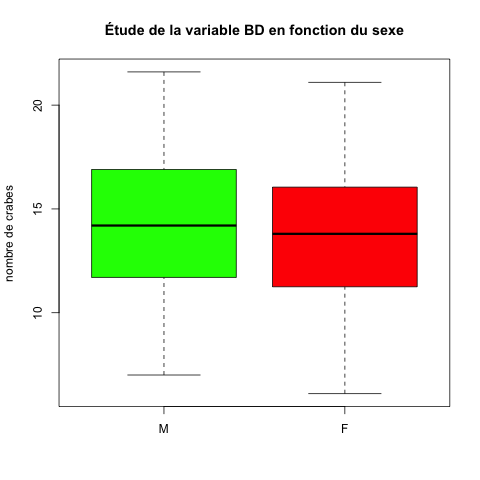
\includegraphics[width=35mm]{Figures/Crabs/bxp_sex_bd.png}
		\end{minipage}
	\end{center}
	
	A l'opposé des boxplot en fonction de l'espèce, ceux en fonction du sexe relèvent une similitude de la distribution des différentes caractéristiques pour la plupart, ainsi que la dispersion des données. Nous observons que la variable RW se distingue des autres avec une largeur de l'arrière importante chez les femmes que chez les hommes.
	
	Enfin, la nature de l'espèce impacte les caractéristiques morphologiques, à la différence du sexe, qui lui n'influe que peu ces caractéristiques.
	
	\subsubsection{Lien entre les variables}
	Nous pouvons représenter chacune de ces variables quantitatives en fonction de l'espèce puis en fonction du sexe afin de déterminer la possibilité d'identifier l'une ou l'autre à partir des caractéristiques morphologiques. \\
	
	\begin{minipage}[t]{0.6\textwidth}
		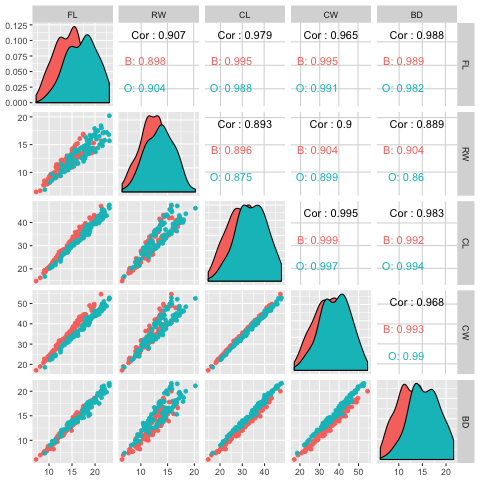
\includegraphics[width=50mm]{Figures/Crabs/matricial_plot_sp.png}
	\end{minipage}
	\begin{minipage}[t]{0.6\textwidth}
		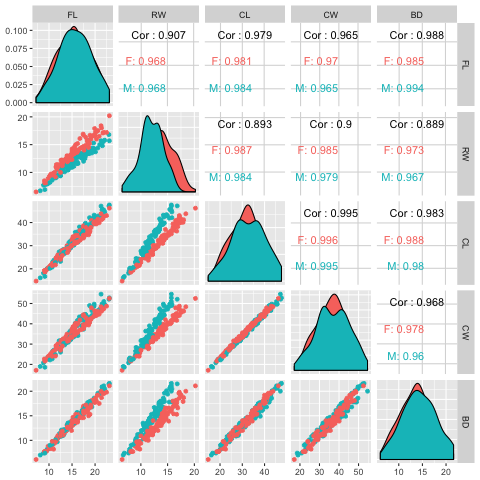
\includegraphics[width=50mm]{Figures/Crabs/matricial_plot_sex.png}
	\end{minipage}
	\begin{center}
		\captionof{figure}{Plot général en fonction de l'espèce (gauche) et du sexe(droite)}
		\label{fig:multiplot_crabs__sp_sex}
	\end{center}
	
	Nous remarquons que ni l'espèce ni le sexe ne peuvent vraiment être identifiés à partir d'une ou de plusieurs caractéristiques morphologiques.
	En effet, dans les deux cas, l'ensemble des points est représenté sur une même droite, on ne peut pas clairement distinguer une différence. De ce fait, il est difficile de reconnaître une espèce selon ses caractéristiques morphologiques.
	
	\subsubsection{Analyse de la corrélation}
	
	\begin{center}
		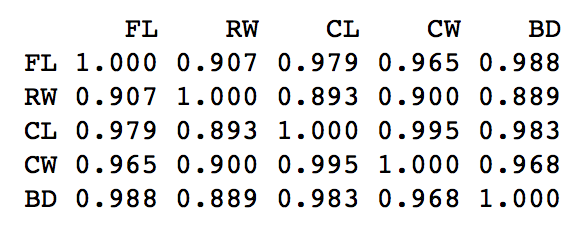
\includegraphics[width=50mm]{Figures/Crabs/cor_crabsquant.png}
		\captionof{figure}{Correlation entre les variables}
		\label{fig:cor_carbsquant}
	\end{center}
	
	Il y a une forte corrélation positive entre toutes les combinaisons de variables, telle que la valeur minimale observée est 0.889. 
	Il s'agit de la taille des membres du corps d'un crabe, il semble donc logique et naturel qu'elles soient proportionnelles entre elles.
	Une des façons pour s'affranchir de ce phénomène est de diviser chaque valeur par la somme totale de toutes celles de l'individu.
	
\subsection{Pima}
Le dataset \textit{"Pima"} représente un jeu de données constitué de 532 individus tous de sexe fémini,n décrits par huit variables dont une qualitative et sept quantitatives.

\subsubsection{Description des variables}

\begin{itemize}
	\item \textbf{Variables Qualitatives Ordinale :}  Pima.z
	\item \textbf{Variables Quantitatives : } Pima.npreg, Pima.glu, Pima.bp, Pima.skin, Pima.bmi, Pima.ped, Pima.age
\end{itemize}

Nous pouvons représenter les données des variables quantitatives à l'aide d'un boxplot normalisé de telle sorte qu'on ait toutes les variables avec une moyenne nulle et une déviation égale a 1.
\begin{center}
	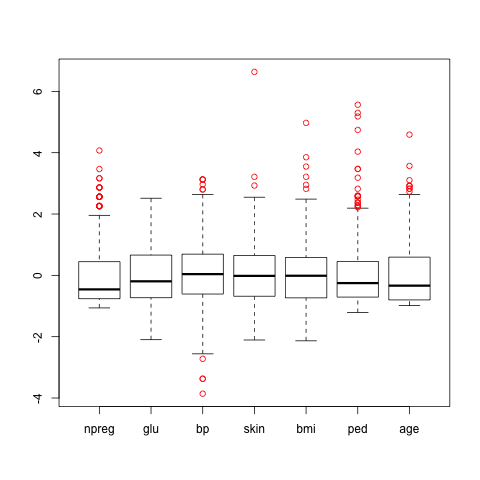
\includegraphics[width=50mm]{Figures/Pima/boxplot_norm_Pimaquant.png}
	\captionof{figure}{Boxplot normalisé des données quantitatives}
	\label{fig:boxplot_norm_pima_quantitatives}
\end{center}

D'après les boxplots normalisés, il existe plusieurs données abérantes. Les variables \textit{ped} et \textit{age} sont clairement pas symétriques. De plus, les distributions des différentes variables sont assez distinctes du fait qu'elles ne se chevauchent pas, ainsi que l'existence de plusieurs valeurs extrêmes.

\begin{center}
	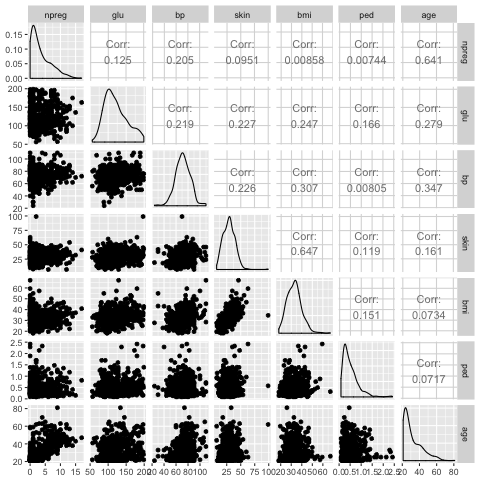
\includegraphics[width=50mm]{Figures/Pima/plot_Pimaquant.png}
	\captionof{figure}{Plot des données quantitatives}
	\label{fig:plot_pima_quantitatives}
\end{center}

Nous remarquons qu'un seul des scartter plots représente une forte association entre l'indice de masse corporelle \textit{bmi} et l'épaisseur du pli cutané au niveau du triceps \textit{skin}.

\subsubsection{Représentation de chaque caractéristique en fonction de z (diabétique ou pas)}

\begin{center}
	\begin{minipage}[t]{0.3\textwidth}
		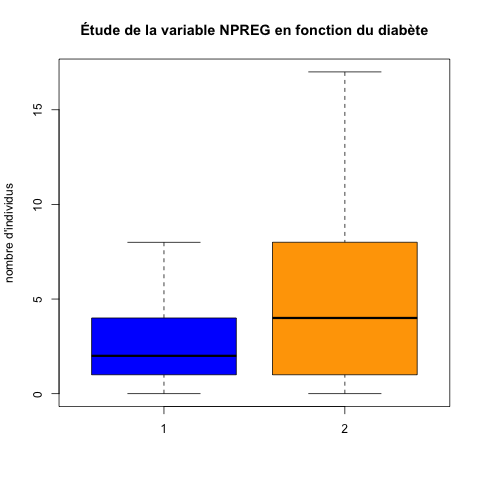
\includegraphics[width=35mm]{Figures/Pima/bxp_z_npreg.png}
	\end{minipage}
	\begin{minipage}[t]{0.3\textwidth}
		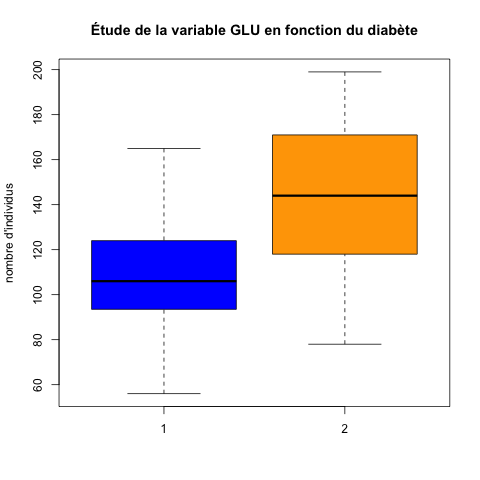
\includegraphics[width=35mm]{Figures/Pima/bxp_z_glu.png}	
	\end{minipage}
	\begin{minipage}[t]{0.3\textwidth}
		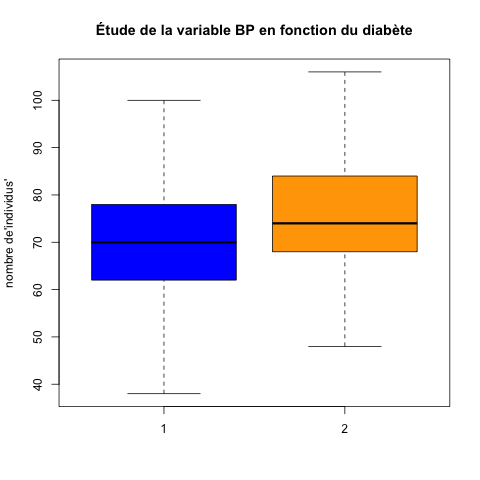
\includegraphics[width=35mm]{Figures/Pima/bxp_z_bp.png}
	\end{minipage}
	\newline
	\begin{minipage}[t]{0.3\textwidth}
		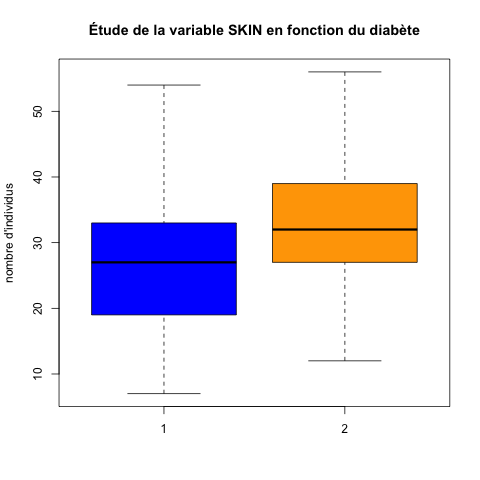
\includegraphics[width=35mm]{Figures/Pima/bxp_z_skin.png}	
	\end{minipage}
	\begin{minipage}[t]{0.3\textwidth}
		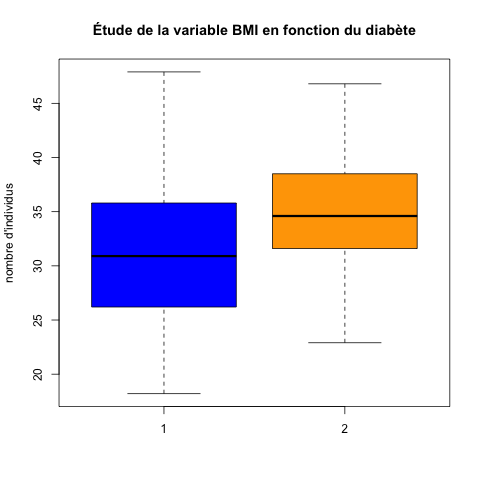
\includegraphics[width=35mm]{Figures/Pima/bxp_z_bmi.png}
	\end{minipage}
	\newline
	\begin{minipage}[t]{0.3\textwidth}
		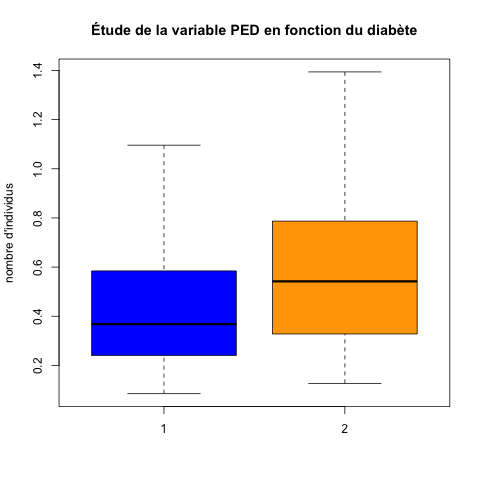
\includegraphics[width=35mm]{Figures/Pima/bxp_z_ped.png}
	\end{minipage}
	\begin{minipage}[t]{0.3\textwidth}
		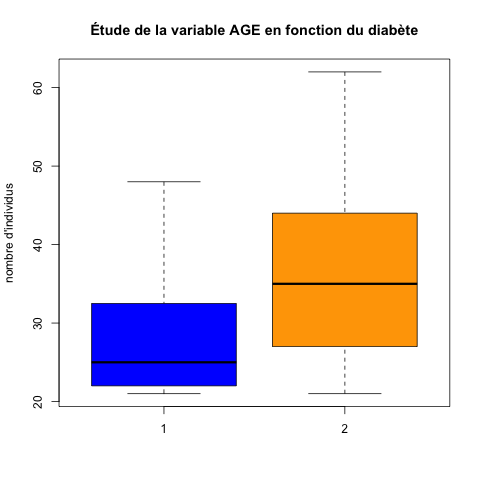
\includegraphics[width=35mm]{Figures/Pima/bxp_z_age.png}
	\end{minipage}
\end{center}

Nous remarquons une grande différence de distributions en fonction de la catégorie \textit{z}. Les intervalles de confiances ne se chevauchent pas. La dispersion des données est aussi différente selon chaque variable. De ce fait, le diabète (variable  qualitative \textit{z}) impacte considérablement chacune des variables quantitatives. 
Selon les médianes bien différentes entre les tests positifs et négatifs de diabète, nous pouvons dire que l'\textit{age} par exemple, la \textit{fonction de pedigree} ou encore le \textit{nombre de grossesses} peut aider à estimer les résultats des tests.
Les données dont on dispose affirment que le diabète ne suit pas forcément la génétique, ceux dont les proches ou ancêtres ont souffert de diabète ne sont pas forcément exposés à un risque élevé d'être affectés eux même. Il est important de noter que cette conclusion ne concerne que le dataset dont on dispose pour cette analyse (elle ne se reflète pas forcement sur les analyses médicales)
	
	\section{Analyse Composantes Principales}
	Dans cette section nous allons nous concentrer sur la technique de l’Analyse en Composantes Principales qui consiste à transformer des variables corrélées en nouvelles variables non corrélées voire aussi à la réduction de dimension.
	\subsection{Exercice théorique}
	Nous travaillons à présent sur les données \textit{notes} mais cette fois-ci les correcteurs sont les individus; et les variables sont : \textit{moy.median, std.median, moy.final, std.final.}. On associe les mêmes pondérations à tous les individus,et on munit $R^{p}$ de la métrique euclidienne. Dans la suite, la matrice M de pondération des variables est la matrice identité.
	\subsubsection{Calcul des axes factoriels de l'ACP}
	Avant de commencer le calcul, nous commençons par centrer notre matrice de données \textit{X.notes} en soustrayant la moyenne de chaque colonne, ce qui permet de mettre le centre de gravité du nuage de points à l'origine. Ceci est possible grâce à la fonction \textit{scale} de R. Tout d'abord, on calcule la matrice des variances \textit{V} par la formule suivante: $V = \frac{1}{6}* X.notes* X.notes^{T}$. Nous obtenons ensuite les valeurs propres $\lambda_{1}, \lambda_{2}, \lambda_{3}, \lambda_{4}$ triées par ordre grâce à la fonction \textit{eigen} ainsi que les vecteurs propres associés. Nous obtenons la matrice U \textit{(ci-dessous)} de vecteurs qui constituent nos axes factoriels de l'ACP.
	
	\begin{center}
		$\lambda_{1}=	1.52 , \lambda_{2}= 1.03, \lambda_{3}= 0.62 , \lambda_{4}= 0.15$
		\[
		U=
		\begin{bmatrix}
		v1	& v2	& v3 &	v4\\
		-0.5691089	& 0.3831062	& -0.4770578 &	0.54932742\\
		-0.6626009	& -0.2607092 &	-0.1954537  &	-0.67438013\\
		0.2342134 & 	0.8173384	&  -0.1888389 & 	-0.49136735\\
		-0.4268714 &	0.3423716 &	0.8357952 &	0.04482142
		\end{bmatrix}
		\]
	\end{center}
	Nous allons à présent calculer le pourcentage cumulé d'inertie expliquée pour chacun des axes v1, v2, v3 et v4. Pour cela on utilise la formule: $P_{k}= \frac{\sum_{i=1}^{k} \lambda_{k}}{\sum_{i=1}^{p} \lambda_{k}}$. Nous obtenons alors l'histogramme ci dessous.
	\begin{center}
		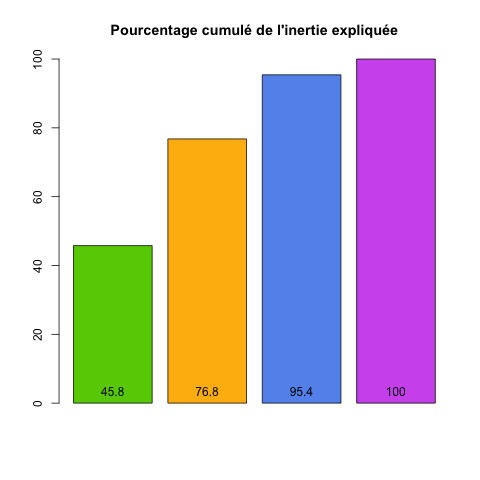
\includegraphics[width=39mm]{Figures/Notes_PCA/pourcentage_inertie.png}
		\captionof{figure}{Pourcentage cumulé de l'inertie expliquée}
		\label{fig:boxplot_crabs_quantitatives}
	\end{center}	
Nous remarquons que les 3 premières composantes ensemble expliquent  95\%  des données, on pourra donc garder que les 3 premiers axes
	
	\subsubsection{Composantes Principales}
	Soit C la matrice  de composantes principale. C s'exprime comme $X.notes.acp = X.notes * U$. Remarquons aussi que la matrice C sera aussi centrée.
	\[
	X.notes.acp=
	\begin{bmatrix}
	c1	& c2	& c3 &	c4\\
	0.1669338 &	-0.8150980	& 0.4438352	& 0.75983420\\
	2.2340546	& 0.9363064	& 0.1554035	& 0.06367979\\
	-0.1186174 &	-0.7571973	& -1.6361255	& -0.05651747\\
	-1.3438493 &	1.8308473 &	-0.1804311 &	0.01407302\\
	0.7303288 &	-0.7032237 &	0.4432574 &	-0.50642647\\
	-1.3349828	& -0.4916345 &	0.7740606 &	-0.27464306
	\end{bmatrix}
	\]
	
	\subsubsection{Représentation des Individus  et variables dans le plan factoriel}
	Afin d'obtenir la contribution de chaque composante dans une variable nous calculons la matrice de corrélation entre l'ancienne matrice des données X.notes et la nouvelle matrice avec les composantes. Ceci se fait grâce à la fonction \textit{corr}. Nous obtenons la matrice de corrélation ci-dessous.\\
	\begin{center}
		\begin{tabular}{c c c c c}
			&	\textbf{moy.median}	&	 \textbf{std.median} &		\textbf{moy.final}	&	\textbf{ std.final}\\
			\textbf{c1}	&	\textbf{-0.775} &		-\textbf{0.90}	&	0.32	&	-0.58\\
			\textbf{c2}	&	0.43 &		-0.29	&\textbf{	0.91}	&	0.38\\
			\textbf{c3}	&	-0.41	&	-0.17	&	-0.16	&	\textbf{0.72}\\
			\textbf{c4}	&	0.23 &		-0.29 &		-0.21	&	0.02
		\end{tabular}
	\end{center}
	On retrouve ici un autre argument comme quoi les 3 premières composantes suffisent pour expliquer les données. En effet les variables sont fortement corrélées aux 3 premières composantes. Nous avons représenté en gras la corrélation la plus forte de chaque variable avec une composante. On peut déduire que la moyenne et l'écart type du médian sont majoritairement expliqués par la composante 1 alors que le la moyenne du final par la composante 2 et pour finir l'écart type du final par la composante 3. La figure suivante \ref{fig:individus_comp}	est une représentation des 6 correcteurs dans le premier plan factoriel (les composantes 1 et 2), alors que la figure \ref{fig:var_comp} représente la contribution de chaque composante pour chacune des 4 variables.
	
	\begin{minipage}{0.5\textwidth}
		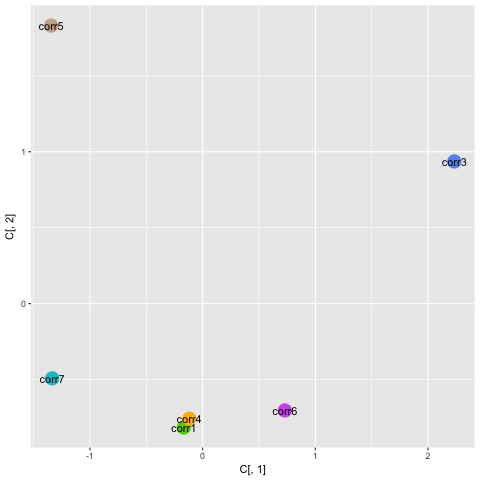
\includegraphics[width=50mm]{Figures/Notes_PCA/individus_comp.png}
		\captionof{figure}{Individus dans le 1er plan}
		\label{fig:individus_comp}	
	\end{minipage}
	\begin{minipage}{0.5\textwidth}
		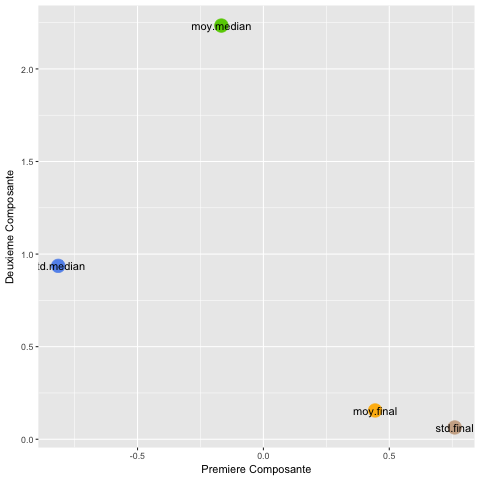
\includegraphics[width=50mm]{Figures/Notes_PCA/variables_comp.png}
		\captionof{figure}{Variables dans le 1er plan}
		\label{fig:var_comp}	
	\end{minipage}
\vspace{0.9mm}
\\La figure \ref{fig:individus_comp} est une représentation de la matrice C et la figure \r est une \ref{fig:var_comp} de la matrice de corrélation dans le premier plan factoriel.
	
	\subsubsection{ Calcul de la matrice X.Notes}
	Dans cette partie nous allons calculer $\sum_{\alpha = 1}^{k} c_{\alpha}u'$ pour k =1, 2, 3 et 4. Pour k= 4 on obtient la matrice \textit{X.notes }. \\
	\begin{minipage}[t]{0.5\textwidth}
	\[
	k=1
	\begin{bmatrix}
	0.09 &	0.11 &	-0.04	& 0.07\\
	-1.27	& -1.48 &	0.52	& -0.95\\
	0.07	& 0.08 &	-0.03	& 0.05\\
	0.76&	0.89 &	-0.31	& 0.57\\
	-0.41	& -0.48 &	0.17	& -0.31\\
	0.760	& 0.88	& -0.31 &	0.57
	\end{bmatrix}
	\]
	\end{minipage}
	\begin{minipage}[t]{0.5\textwidth}
	\[
		k=2
		\begin{bmatrix}
		-0.22 &	0.32 &	-0.70 &	-0.21\\
	-0.91 &	-1.72 &	1.29 &	-0.63\\
	-0.22 &	0.28 &	-0.65 &	-0.21\\
	1.47 &	0.41 &	1.18 &	1.20 \\
	-0.60 &	-0.30 &	-0.40 &	-0.55\\
	0.57&	1.01 &	-0.71	& 0.40	
		\end{bmatrix}
	\]
	\end{minipage}



\begin{minipage}[t]{0.5\textwidth}
	\[
	k=3
	\begin{bmatrix}
	-0.43 &	0.24 &	-0.80 &	0.16\\
	-0.99 &	-1.75 &	1.26 &	-0.50\\
	0.56 &	0.60 &	-0.34 &	-1.58\\
	1.55&	0.45 &	1.22 &	1.05\\
	-0.90 &	-0.39 &	-0.49 &	-0.18\\
	0.20 &	0.86  &	-0.86 &	1.05
	
	\end{bmatrix}
	\]
\end{minipage}
\begin{minipage}[t]{0.5\textwidth}
	\[
	k=4
	\begin{bmatrix}
	-0.01	& -0.28& 	-1.16	&  0.20\\
	-0.95	&  -1.80 & 	1.23 & 	-0.50\\
	0.53 & 	0.63 & 	-0.31	&  -1.58\\
	-1.17	& -0.045 &	-0.24	& -0.20\\
	0.05 &	1.05 &	-0.73 &	1.04
	
	\end{bmatrix}
	\]
\end{minipage}

\subsubsection{Représentation des individus initialement écartés de l’ACP}
Dans cette sous partie nous allons nous intéresser aux 2 correcteurs qu'on a omis au début de l'étude parce que certaines de leurs variables n'étaient pas définies. On a d'abord mis à 0 les NA pour chacun des correcteurs puis nous avons effectué une imputation par la moyenne, en remplaçant chaque valeur non définie par la moyenne de la variable. Nous obtenons ainsi la sous matrice centrée \textit{X.Notes.imput} suivante:\\

\begin{tabular}{c c c c c}
	Correcteur & moy.median &	std.median	& moy.final	&std.final\\
	Cor2 & 1.63 &	-0.44 &	-1.28 &	-1.04\\
	Cor3 & -1.52 &	-0.84 &	0.53 &	-1.46
\end{tabular}
\vspace{0.9mm}
\\Pour obtenir les composantes de ces 2 individus nous n'avons pas à refaire tous les calculs mais juste à calculer $X.Notes.imput C$ avec C notre matrice de composantes calculée précédemment. Nous obtenons les résultats suivants:\\

\begin{minipage}[t]{0.5\textwidth}
\begin{tabular}{l l l l l}
	Cor &  c1         &             c2 &          c3               &  c4\\
	Cor2 & -0.49 &	-0.66&	-1.31 &	1.78\\
	Cor3 & 2.16	& -0.43  &	-0.43& 	-0.59
\end{tabular}
\end{minipage}
\begin{minipage}[t]{0.5\textwidth}
		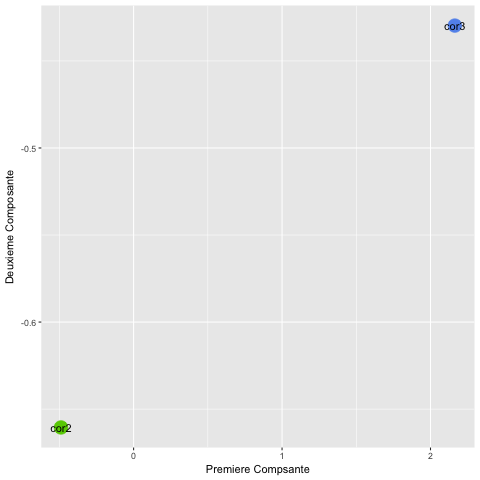
\includegraphics[width=50mm]{Figures/Notes_PCA/individus_comp_na.png}
	\captionof{figure}{Cor2 et Cor3 dans le 1er plan}
	\label{fig:individus_comp_na}	
\end{minipage}

On peut déduire de part notre étude préalable que le correcteur 2 "aurait" une moyenne et un écart type de médian faible (car composante 1 faible) alors que le correcteur 3 a une moyenne de final élevée.

\subsection{Crabs}
\subsubsection{ACP sans traitement préalable}
	Nous faisons appel a la fonction \textit{princomp }qui calcule les composantes principal de notre dataset. Ensuite nous utilisons la commande  \textit{\textbf{crabs.pca\$sd$\string^$2}}   pour obtenir les valeurs propres et représenter le pourcentage d'inertie cumulée dans la figure \ref{fig:crabs_pca_plot}. Le biplot dans la figure \ref{fig:crabs_pca_biplot}.\\
	\begin{minipage}{.5\textwidth}
		\centering
		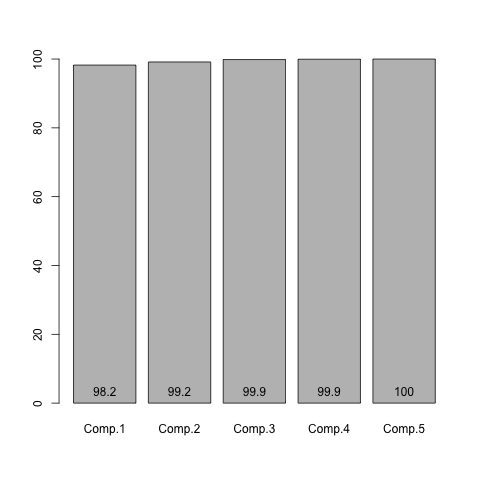
\includegraphics[width=50mm]{Figures/Crabs/pca_plot.png}
		\captionof{figure}{Variance expliquee par les composantes}
		\label{fig:crabs_pca_plot}
	\end{minipage}%
	\hspace{0.08\linewidth}
	\begin{minipage}{.5\textwidth}
		\centering
		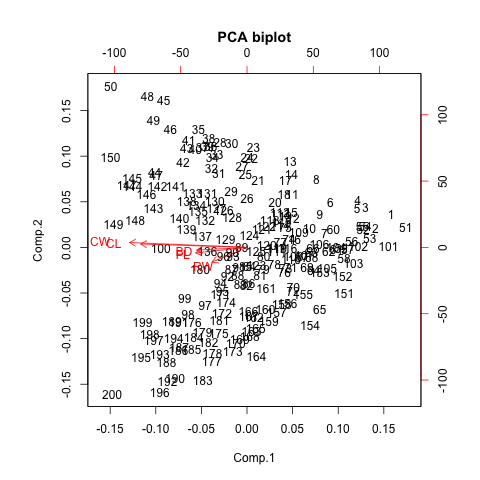
\includegraphics[width=50mm]{Figures/Crabs/pca_biplot.png}
		\captionof{figure}{Individus et Variables projetes sur le premier plan factoriel}
		\label{fig:crabs_pca_biplot}
	\end{minipage}
	\vspace{2mm}
	
	D'après la figure \ref{fig:crabs_pca_biplot}, on remarque que la première composante concentre la majorité de l'information, ceci est aussi illustré dans la figure \ref{fig:crabs_pca_plot} puisqu'on remarque que toutes les variables sont 'encodees' dans la composante 1. D'après notre étude dans la partie analyse des données, nous avons remarqué que les variables sont fortement corrélées et donc proportionnelles. Or l'une des conditions d'utilisation de l'ACP est que les variables soit décorrélees. Ainsi pour de meilleurs résultats, on essayera dans la question qui suit de décorréler les variables et retenter l'ACP.
	
	\subsubsection{Solution proposée}
	Afin d'obtenir des variables non corrélées, nous avons divisé chaque donnée d'une ligne par la somme des valeurs de la ligne. Ensuite comme nous souhaitons étudier l'espèce et le sexe nous avons pensé qu'il serait mieux de regrouper ces 2 résultats en un afin d'obtenir une variable 'réponse' qui prend 4 valeurs; par exemple la valeur \textit{BF} signifie crabe d'espèce B et de sexe Femelle. Les instructions sont détaillées dans le fichier de code en annexe. Le graphe matriciel  ci-dessous montre les résultats obtenus.
	
	\begin{center}
		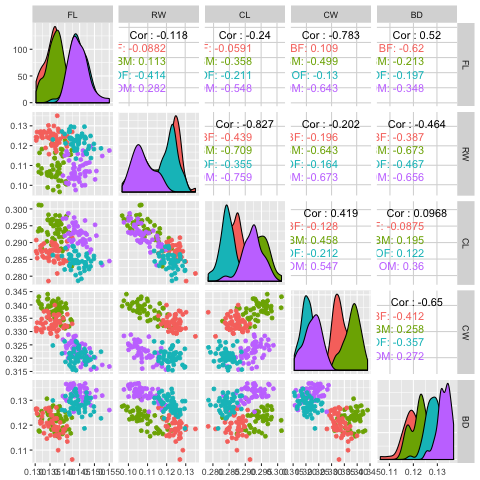
\includegraphics[width=50mm]{Figures/Crabs/matricial_plot_decorr_classes.png}	
		\captionof{figure}{Plot Matriciel des caracteristiques apres decorelation}
		\label{fig:crabs_matricial_plot_decorr}
	\end{center}

	On remarque qu'a présent on peut visiblement distinguer les espèces par leur caractéristiques. Par exemple si on observe le plot de  "RW" en fonction de "CW" les espèces sont séparées.\\
	
	A présent nous pouvons réaliser une ACP sur ces données. Nous obtenons les résultats suivants:
	
	\begin{minipage}{.5\textwidth}
		\centering
		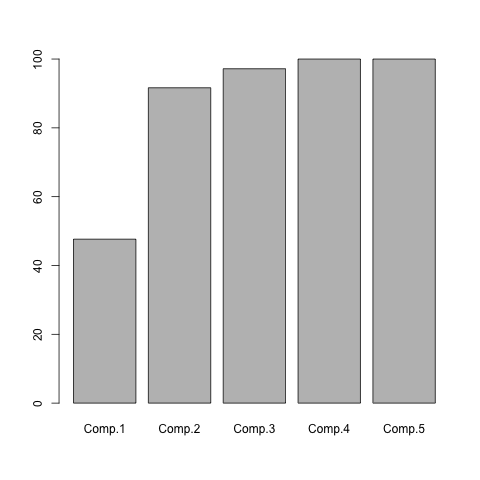
\includegraphics[width=50mm]{Figures/Crabs/decorr_pca_plot.png}
		\captionof{figure}{Variance expliquee par les composantes apres decorrelation}
		\label{fig:crabsd_pca_plot}
	\end{minipage}%
	\hspace{0.08\linewidth}
	\begin{minipage}{.5\textwidth}
		\centering
		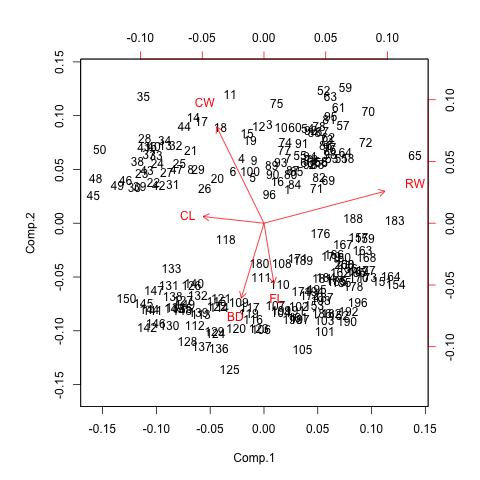
\includegraphics[width=50mm]{Figures/Crabs/decorr_pca_biplot.png}
		\captionof{figure}{Individus et Variables sur le 1er plan factoriel apres decorrelation}
		\label{fig:crabsd_pca_biplot}
	\end{minipage}
	
	\vspace{2mm}
	La figure  \ref{fig:crabsd_pca_biplot} nous montre que les variables RW et OL sont contenues principalement dans la composante 1 alors que les variables BO, FL et CW seront plus dans la composante 2. Ce qui est aussi affiché dans la \ref{fig:crabsd_pca_plot} vu que les 2 premières composantes ensemble concentrent le maximum de variance expliquée. Enfin, la même figure nous permet aussi de conclure que la \textbf{l'information sur le sexe se trouve dans la composante 1 tandis que la composante 2 contient l'information sur l'espèce du crabe}. 
\subsection{Pima}

\subsubsection{ACP}

Nous utilisons la fonction princomp pour calculer les composantes principales dans ce dataset après avoir centré en colonne les données. Ensuite nous représentons le plot et le biplot comme suit:
\\
\begin{minipage}{.5\textwidth}
	\centering
	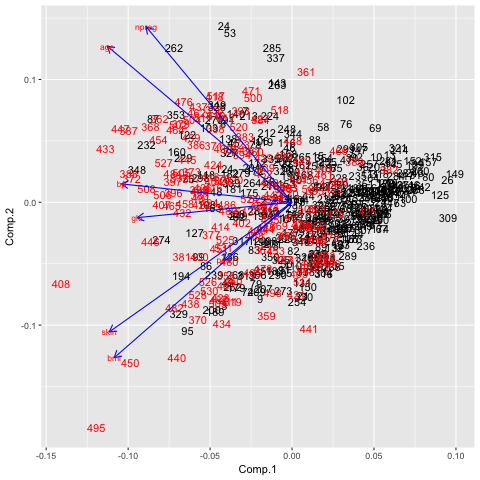
\includegraphics[width=50mm]{Figures/Pima/pca_plot.png}
	\captionof{figure}{Variance expliquée par les composantes}
	\label{fig:pima_pca_plot}
\end{minipage}%
\hspace{0.08\linewidth}
\begin{minipage}{.5\textwidth}
	\centering
	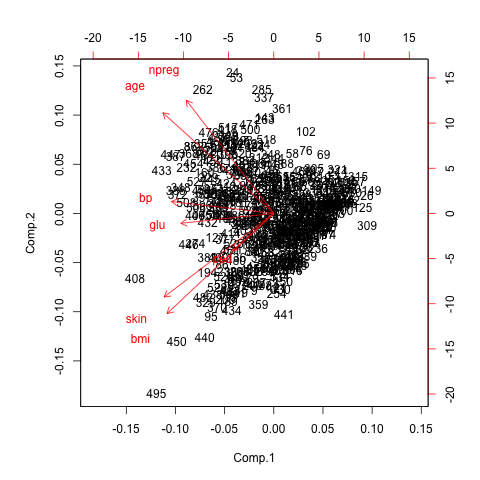
\includegraphics[width=50mm]{Figures/Pima/pca_biplot.png}
	\captionof{figure}{Individus et Variables projetées sur le premier plan factoriel}
	\label{fig:pima_pca_biplot}
\end{minipage}
\\
\\
Pour connaître le comportement général du dataset, nous pouvons considérer les 80\% des pourcentages cumulés. Dans ce cas, nous prenons 4 composantes. Si on s'intéresse aux détails et qu'on va jusqu'à une inertie de 95\%, on remarque qu'il faudra prendre 6 composantes. En effet, les variables sont très indépendantes et fortement decorrélées. Le seul cas où on peut avoir une représentation simple est le cas général de 80\%, autrement on ne diminue pas énormément la dimension. De ce fait, nous ne pouvons pas vraiment avoir une représentation simple pour distinguer les deux catégories de patientes.
	
	\section{Conclusion}
	Ces différents exercices nous ont permis d'abord de manipuler différentes données et de se familiariser avec la notion de variable qualitative et quantitative pour mieux représenter les données graphiquement. Nous avons passé le plus de temps possible dans la première partie afin de mieux comprendre les fonctionnalités du \textit{R} et surtout de \textit{ggplot}, ce qui a facilité notre analyse. Nous avons ensuite utilisé la méthode de l'\textit{ACP} qui est très utile pour l'obtention d'axes decorrélés. Enfin si nos variables sont corrélées on peut avoir des valeurs propre nulles et donc un nombre petit de composantes. L'\textit{ACP} est aussi fortement utilisée dans la réduction de dimension, ce qui fera sujet de nos prochaines études en SY09. 
\end{document}
